\section{Evaluation}\label{sec:eval}

In order to measure how interesting and interactive our \tube is, we developed our applications to be able to accept inputs from both traditional input devices (\ie mouse and keyboard) and our \tube. For instance, in the balloon popping game, the user will be able pop the balloons by clicking them with the mouse. To match the balloons’ colors, the users will have to press the appropriate keys on the keyboard. After describing to our participants how our \tube works, the participants tried out the applications that we have developed with mouse and keyboard first, and later with the \tube as the input device.

The first thing that our testers did when trying out the \tube was figuring out how to control the small pointer on the screen. Since pointer in the screen is moving correspondingly as our testers played around with \tube, our testers adapted to the system naturally and in no time successfully played with our \tube. Additionally, we have also observed the bursting animation and sound that is generated whenever a balloon is popped gave the users a sense of accomplishment.

\begin{figure}
  \centering
  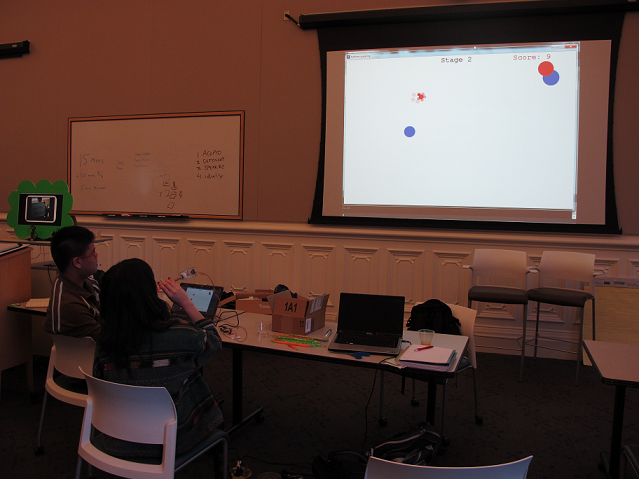
\includegraphics[width=\linewidth]{./figs/impl2.png}
  \caption{Our testers trying out \tube during a project showcase at UC Berkeley campus.}
  \label{fig:impl2}
\end{figure}

\marginpar{
\begin{figure}
  \begin{center}
  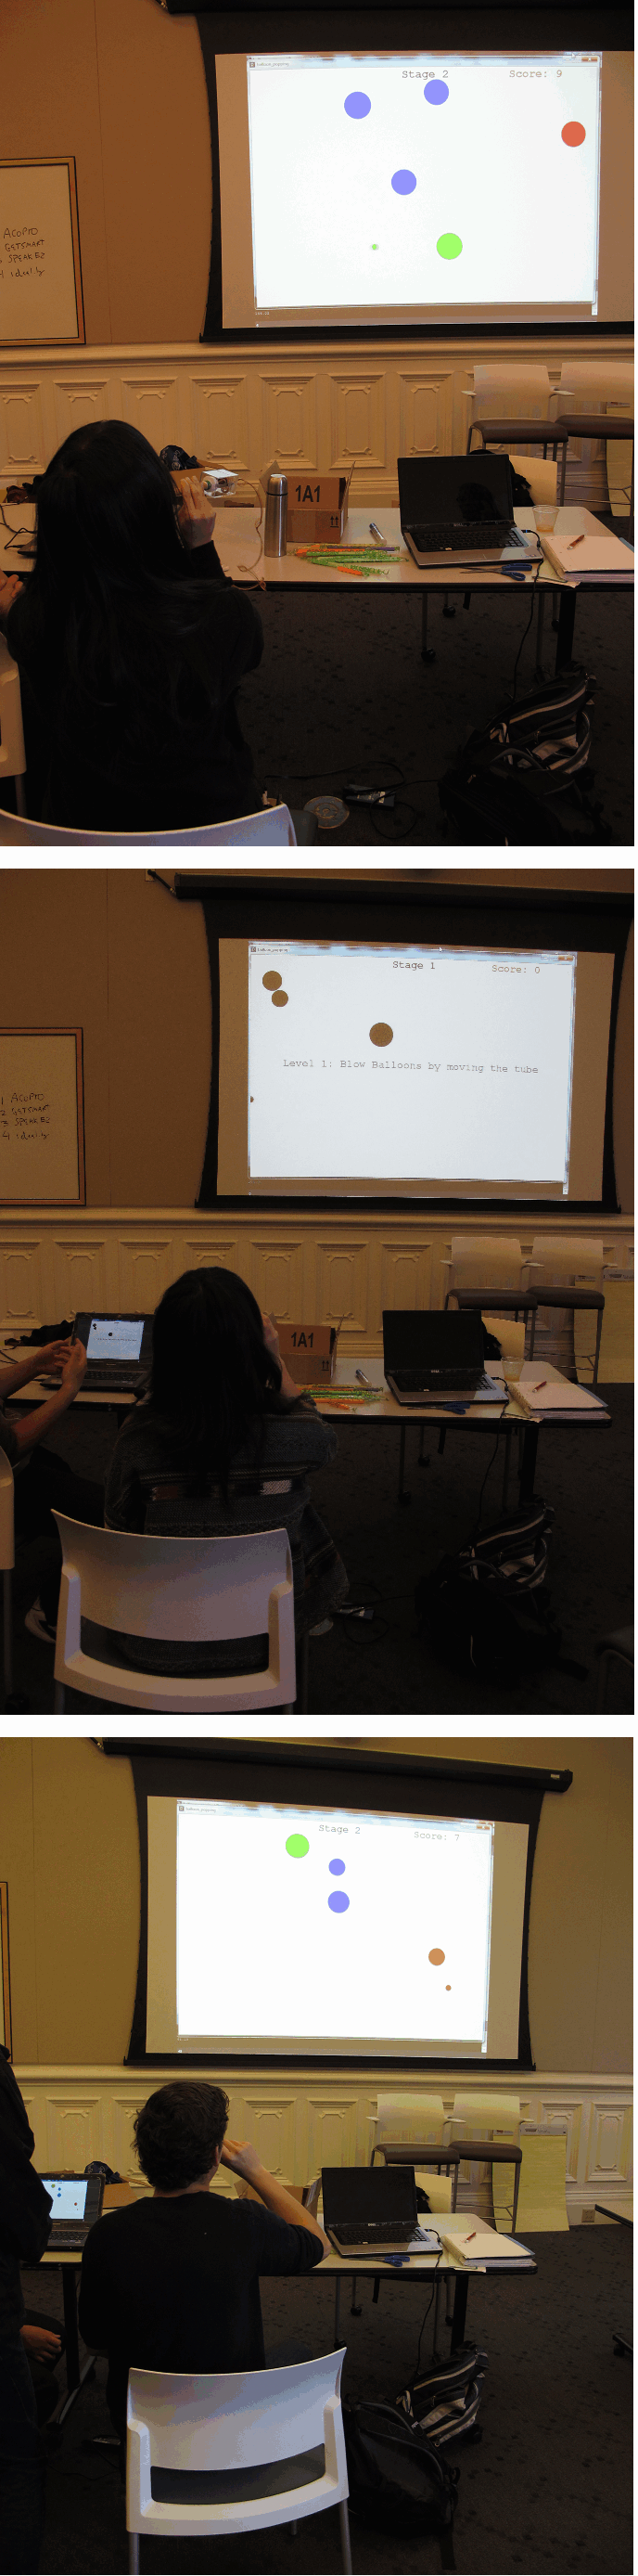
\includegraphics[width=0.7\marginparwidth]{./figs/eval.png}
  \label{fig:eval}
  \end{center}
\end{figure}
}

The challenging part is when the users have to match the color of the pointer with the color of the balloon by rotating the tube. It is not that obvious for our testers that they needed to rotate \tube in order to change the color of the pointer for this type of interaction is one of a kind. In the second level of our balloon popping game, after observing that they could not pop the balloon through blowing into the tube only, they started experimenting with orienting \tube in different positions and noticed that the color of the pointer changes. However, after some time, our testers eventually grasped this distinct feature of our \tube and continue to enjoy the rest of the game.

% G flow:
% However, we may need to improve on our hardware design since some users lamented on the motion sensitivity of our \tube.
